\documentclass[12pt]{article} % for thesis

% \usepackage[top=0.5in, bottom=0.5in, left=0.5in, right=0.5in]{geometry}
% \documentclass[twocolumn,9pt]{article}
\usepackage{spconf}
\usepackage[utf8]{inputenc}
\usepackage{natbib}
\usepackage{graphicx}
\usepackage{stfloats} % for positioning of figure* on the same page
\usepackage{caption}
\usepackage{tikz}
\usepackage[inline]{enumitem}
\usepackage{amsmath}
\usepackage[breaklinks=true,colorlinks=true, allcolors=blue]{hyperref}
\usepackage{breakcites}
\usepackage{microtype}
\usepackage{lipsum}
\usepackage{xcolor}
\usepackage{array}
\usepackage{float}
\usepackage{adjustbox}
\usepackage{listings}
\usepackage{csquotes}
\usepackage{makecell}
\usepackage{pdfpages}
\usepackage{xspace}
\usepackage{tikz}

\usetikzlibrary{positioning,shapes.geometric}

% to do:
% hearing tests
% one other way to present results is grouped by which losses are most appropriate for each situtation

\usepackage{xcolor}
\usepackage[utf8]{inputenc}       % For UTF-8 encoding
\usepackage{listings}
\usepackage{amsmath}              % Optional: for math symbols
\usepackage{anyfontsize}
\usepackage{graphicx} % required for \scalebox

\lstdefinelanguage{Faust}{
    morekeywords={import, process, environment, declare, with, if, else, while, for, int, float, true, false},
    sensitive=true,
    morecomment=[l]{//}, % Line comment
    morecomment=[s]{/*}{*/}, % Block comment
    morestring=[b]", % Strings
}

% Customize the appearance of the code
\lstset{
    language=Faust,
    backgroundcolor=\color{lightgray!20},
    % basicstyle=\ttfamily\small,
    basicstyle=\fontsize{8pt}{9pt}\selectfont\ttfamily,
    keywordstyle=\color{blue}\bfseries,
    stringstyle=\color{orange},
    commentstyle=\color{green}\itshape,
    showstringspaces=false,
    % numbers=left,
    % numberstyle=\tiny,
    frame=single,
    breaklines=true,
      % basicstyle=\ttfamily,
  % literate={\delta}{{\(\delta\)}},
}


\captionsetup[lstlisting]{justification=centering, singlelinecheck=false}
\providecommand{\gls}[1]{#1}
\newcommand{\highlight}[1]{\textcolor[RGB]{00,150,00}{#1}}
\newcommand{\todo}[1]{\textcolor{red}{#1}}

\newcommand{\SIMSESpec}{\texttt{SIMSE\_Spec}\xspace}
\newcommand{\LoneSpec}{\texttt{L1\_Spec}\xspace}
\newcommand{\JTFS}{\texttt{JTFS}\xspace}
\newcommand{\DTWEnv}{\texttt{DTW\_Envelope}\xspace}
\newcommand{\OutDomain}{\textbf{Out-of-Domain Generation}\xspace}
\newcommand{\LossSelect}{\textbf{Loss Selection}}
\newcommand{\SynthSelect}{\textbf{Synthesis Selection}}
\newcommand{\PeriodicLoss}{\textbf{Periodic Loss}}

\newcommand{\BPNoise}{\textbf{BP-Noise}\xspace}
\newcommand{\BPSaw}{\textbf{BP-Saw}\xspace}
\newcommand{\AddSineSaw}{\textbf{Add-SineSaw}\xspace}
\newcommand{\AmpMod}{\textbf{Noise-AM}\xspace}
\newcommand{\FMMod}{\textbf{SineSaw-AM}\xspace}
\newcommand{\FMModvtwo}{\textbf{SineSine-AM}\xspace}
\newcommand{\PitchBendUp}{\textbf{PitchBend-Up}\xspace}

\title{Selecting Loss Functions for Out-of-Domain Sound-Matching}
\begin{document}

\name{Amir Salimi, Abram Hindle, Osmar R. Za{\"i}ane}
\address{University of Alberta}

\maketitle

%     Despite their critical role in sound-matching, the performance of different sound-similarity measures (or loss functions) under different circumstances has rarely been a topic of research. Should we be looking for a global sound-similarity measure, or is the choice of loss function a creative decision, much like the selection of a synthesizer?

\begin{abstract}
 Out-of-domain sound-matching is the task of automatically programming a synthesizer towards a sound that it cannot accurately replicate. While this approach to sound-matching is far better suited for practical applications to design, it has rarely been explored. Measuring performance in out-of-domain sound-matching is a difficult task due to the subjective experience of sound, open-set recognition, characteristics of interest, et cetera. In addition, despite their critical role in sound-matching, the performance of different sound-similarity measures (or loss functions) under different circumstances has rarely been a topic of research. Should we be looking for a global sound-similarity measure, or is the choice of loss function a creative decision, much like the selection of a synthesizer?
 Here we present a series of differentiable out-of-domain sound-matching scenarios using four loss functions and various synthesizers. The experiments here are designed such that differences in parameters (whether all parameters or a subset) are well suited for measuring performance in sound-matching. The out-of-domain experiments here showcase the characteristics of the different loss functions, and confirm that their success is highly dependent on the method of synthesis and the target sound. 
\end{abstract}

\section{Experiment Overview}
\begin{itemize}
    \item $g(\theta)$: A parametric audio synthesizer $g$ with parameters $\theta$. The corresponding sound is $x$, or $g(\theta) = x$. 
    \item $g^{t}(\theta^t)$: The target synthesizer $g^{t}$ outputs the target sound $x^t$. The corresponding sound (or \textit{target} sound) is $x^t$. For experiments to be OOD, $g^t$ and $g$ must be designed differently, or have non-overlapping parameter ranges such that $ g(\theta) \neq g^t(\theta^t)$ for any $\theta$.\
    
     % (if we denote $\forall x \in \mathcal{X}$ and $\forall x^t \in \mathcal{X}^t$ then $\mathcal{X}^t\cap\mathcal{X}=\emptyset$).
    \item $x_\theta$: The synthesizer output given a set of parameters $\theta$, $x_\theta = g(\theta)$”.
    \item $x^t$: The target sound to be replicated or imitated. 
    \item $\phi(\cdot)$: A representation (feature extraction) function mapping signals into a comparison space.
    \item $L$: A loss function that measures distance between $x_\theta$ and $x^t$, typically via $L(\theta,x^t) = d(\phi(x_\theta), \phi(x^t))$ for some metric $d$.
\end{itemize}

\begin{figure}[ht]
    \centering
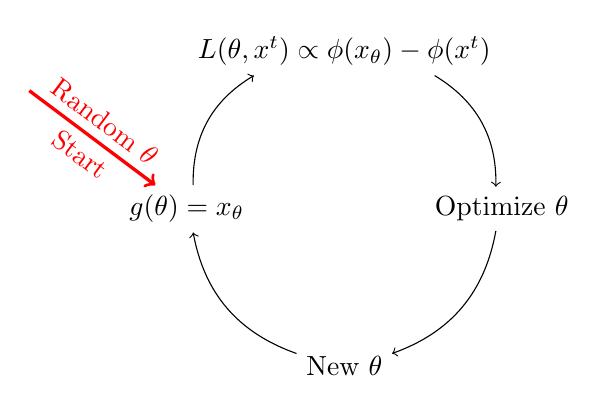
\begin{tikzpicture}[node distance=2cm, auto]

% Nodes
\node (start) [text centered] {\( g(\theta) = x_{\theta} \)};
\node (L) [above of=start, right of=start, text centered] 
    {\( L(\theta, x^t) \propto \phi(x_{\theta}) - \phi(x^t) \)};
\node (optimize) [below of=L, right of=L, text centered] {Optimize $\theta$};
\node (new_theta) [below of=optimize, right of=start, text centered] {New \( \theta \)};

% Highlight and arrow for the start node
\draw[->, very thick, red] (start) ++(-2,1.5) -- (start)
    node[midway, below, align=center, sloped, color=red] {Start}
    node[midway, above, align=center, sloped, color=red] {Random $\theta$};

% Arrows with multi-line labels
\draw[->, bend left] (start) to node[midway, right, align=center] {} (L);
\draw[->, bend left] (L) to node[midway, right, align=center] {} (optimize);
\draw[->, bend left] (optimize) to node[midway, below, align=center] {} (new_theta);
\draw[->, bend left] (new_theta) to node[midway, left, align=center] {} (start);

\end{tikzpicture}
    % \caption{ Iterative approach to sound design. Synthesizer $g$ with arbitrary initialized parameters $\hat{\theta}$, creates sound $x$. The target sound $t$ is used as the goal. Parameters $\hat{\theta}$ are adjusted to minimize error (or loss) $L(\hat{\theta},t)$, where $L$ is proportional to the difference between the representations of $x$ and $t$. $\phi$ is the audio feature extractor, or representation function.}
    \caption{ Iterative approach to sound design. Adapted to OOD scenarios~\cite{salimi2025evaluating}.}
    \label{fig:sound_design_loop_iterative}
\end{figure}


\section{Performance Measures}
Manual sound-design is a feedback loop built on the designer hearing an output and measuring the similarity of what is currently generated versus what they would like to hear. This subjective, internal measurement of sound qualities is impossible to recreate between people with similar tastes, let alone digitally. Over the years, many automatic performance measure have been used in previous work, but the generality of such results from such experiments have generally viewed with a large degree of skepticism~\todo{cite}. This is because such experiments have largely been conducted in the in-domain setting, where perfect matching between the target and output sounds ($x^t$ and $x_\theta$), or target and output parameters ($\theta^t$ and $\theta$) is possible. In such cases, reaching the value of zero in L1 or MSS difference of the spectrograms of sounds or the L1 difference between the parameters (i.e., P-Loss) has been a common performance measure. 

In OOD experiments, the usual automatic measures of performance are not applicable. While the subtraction of spectrograms (whether L1, L2, or MSS) can show whether or not two sounds are near identical, larger values in these measures does not correlate with larger differenes~\cite{turian2020sorry,vahidi2023mesostructures}. In addition, P-Loss requires identical parameter sets between synthesizers, which by definition cannot be applied in OOD scenarios. 

In this work we use manual listening tests, which are the gold standard for measuring performance in sound-matching. After all, assistance with manual sound-matching is the most common stated goal of previous sound-matching work~\todo{cite}. In addition, we propose partial P-Loss (PPL), as a reasonable automatic measure of sound-matching performance in out experiments, show whether it correlates with manual listening tests. 



\section{methodology}
The foundation of our experiments is the iterative loop shown in Figure~\ref{fig:sound_design_loop_iterative}. This iterative approach is the OOD adaption of previous work by Salimi \textit{et al.}~\cite{salimi2025evaluating}. The goal of the experiments here is to measure the performance of loss functions in different OOD \textit{scenarios}. Each scenario tells us about the effectiveness of loss functions in matching sounds of a certain characteristic. In each scenario, the synthesizers are unchanged, with variation in the loss functions. 

The definition of an experiment requires that $g^t$, $g$, the loss function $L$, and max number of iterations $n$ are fixed. Each experiment has three phases
\begin{enumerate}
    \item Create a target sound $x^t$ by with random parameters $\theta^t$ given to $g^t$. $g$ is also randomly initiated with $\theta_n$, where $n$ indicates the number of iterations, beginning at $n=0$
    \item Iteration through the loop, where the distance between the target sound $x^t$ and the the synthesizer's output is measured by $L$, and $\theta$ is updated.
    \item After $n$ number of iterations, a \textit{performance measure} is used to measure success by comparing the $x^t$ to the final output of the synthesizer. 
\end{enumerate}




\clearpage
\bibliographystyle{alpha}

\bibliography{references}

\end{document}
